\documentclass{article}
\pdfpagewidth=8.5in
\pdfpageheight=11in

\usepackage{ijcai27}

\usepackage{times}
\usepackage{soul}
\usepackage{url}
\usepackage[hidelinks]{hyperref}
\usepackage[utf8]{inputenc}
\usepackage[small]{caption}
\usepackage{graphicx}
\usepackage{amsmath}
\usepackage{amssymb}
\usepackage{amsthm}
\usepackage{booktabs}
\usepackage{xcolor}
\usepackage[switch]{lineno}

% Comment out this line in the camera-ready submission
\linenumbers

\urlstyle{same}

\newcommand{\Safe}{\textsc{safe}}
\newcommand{\Unsafe}{\textsc{unsafe}}
\newcommand{\Description}[1]{}
\DeclareRobustCommand{\citep}[1]{\cite{#1}}
\DeclareRobustCommand{\citet}[1]{\citeauthor{#1}~\shortcite{#1}}

\pdfinfo{
/TemplateVersion (IJCAI.2027.0)
}

\title{Self-Play Rates Are Not Risk Profiles:\\Five LLM Endpoints Against Fixed Rivals in an AI Race}

\author{
    Anonymous Submission
}

\begin{document}

\maketitle

\begin{abstract}
A language-model agent's response to risk in self-play describes a pairing, not
the agent, because its rival is an adapting copy of itself. We show this in an
idealised AI-development race, where faster \Unsafe{} development raises the
winner's chance of losing its payoff. Five commercial endpoints that passed a
frozen task-validity screen played four fixed, undisclosed rival policies at
three risk levels, with ten matched race blocks per cell and a second block for
the two unconditional rivals. All five play more \Unsafe{} against an
always-\Unsafe{} rival, as any best responder would. The rival-by-risk
interaction is more informative, because an informed best response predicts a
positive sign and a noisy best response fitted to each endpoint predicts a
negative one. Claude Sonnet 5 falls inside its noisy benchmark, Gemini 3 Flash
and GPT-5.4 are near zero, and Claude Opus 5 and GPT-5.5 show the positive sign,
which the fitted noisy benchmark excludes. Claude Sonnet 5 run with reasoning
enabled, the decoding setting Opus and GPT-5.5 use, turns more negative, so
reasoning alone does not produce the positive sign. A self-play rate therefore
does not identify an endpoint's response to risk. Claims are scoped to five
endpoints, one prompt rendering and one idealised game.
\end{abstract}

\section{Introduction}
\label{sec:introduction}

Self-play is attractive because it is symmetric and easy to reproduce. It is
also a compound measurement: the evaluated endpoint is both the focal agent and
the environment to which that agent reacts. When a treatment changes behaviour,
the observed rate may therefore reflect two adapting copies rather than a stable
property of either one. This matters for language models used in strategic
settings, where responses to an opponent can be exactly what the evaluation is
trying to distinguish from responses to risk
\citep{lekeasNashSuppression2026,herrStrategicBias2024,playing_repeated_games_with_llms}.

We study this identification problem in an idealised race over AI development. Each
round, two agents choose between slower \Safe{} development and faster
\Unsafe{} development; \Unsafe{} creates a delayed chance that the winner loses
its payoff. The game represents a controlled speed and safety dilemma rather than a
real company in full \citep{ai_race_for_strategic_advantage,racing_to_the_precipice}.
A broader AI-race literature models bidding incentives, heterogeneous actors,
regulation and voluntary safety commitments
\citep{han2019modelling,to_regulate_or_not,artificial_intelligence_development_races,han2022voluntary};
scenario games likewise identify coordination as central to race outcomes
\citep{gruetzemacher2025strategic}.
Its value is experimental: stated danger, rival policy and progress can be held
fixed separately. We reproduce the two-player mechanism of
\citet{falling_behind_unsafe}. One hosted model at one fixed configuration is an
\emph{endpoint}; model families can differ across dated versions and provider
settings.

LLM behavioural research now spans cognitive benchmarks and repeated
matrix games \citep{codaFornoCogBench2024,playing_repeated_games_with_llms},
reproducible testbeds with language and payoff interventions
\citep{buscemiFAIRGAME2025,huynhUnderstanding2025,huynhPayoffScaling2026}, and
multi-agent common-resource societies \citep{piattiGovSim2024}.
Game-theoretic benchmarks run LLM-versus-LLM competitions
\citep{duanGTBench2024}, repeated-game studies pair models with human-like
fixed strategies \citep{playing_repeated_games_with_llms}, and evolutionary
tournaments pit models against canonical strategies
\citep{payneStrategicIntelligence2025}. Outcomes also change sharply when the
interaction partner changes \citep{lekeasNashSuppression2026}. As far as these
reports show, none of them crosses a fixed, undisclosed rival with a stated
catastrophe risk in a paired design whose rival moves are recomputed from the
recorded history, and none compares the result with the informed best response to
that rival. That is the gap we fill. Our question is narrower than general
strategic skill: \emph{when the mirror opponent is replaced by a fixed policy,
how far is the response to the stated catastrophe risk from the best response to
that policy?} That is the estimand a safety reading needs, and a high or low
self-play rate alone cannot answer it.

Two checks protect this inference. First, a valid action format does not prove
that an endpoint tracked state, arithmetic or terminal scoring. We use a frozen
operational inclusion rule and let the game engine, rather than generated text,
resolve every transition. Second, even equivalent prompt renderings can change
model output in strategic games
\citep{robinsonBurdenFraming2025,mousaviDavoudiEtAl2026}. More generally,
formatting and answer order matter
\citep{sclarPromptFormatting2024,pezeshkpourOptionOrder2024,weiSelectionBias2024},
as do small prompt and persona changes
\citep{salinasButterfly2024,zhengPersona2024,herrStrategicBias2024}.
We therefore separate frozen-protocol gameplay from presentation diagnostics and
retain the prompt, raw response, parsed action, state and terminal record for
every decision.

The answer is not one universal opponent effect. In self-play, every included
endpoint reduces \Unsafe{} play as stated risk rises, with four graded profiles
and one threshold-like switch. Against four fixed scripted rivals, all five
endpoints move substantially with the rival, as a best-responding agent would.
The informative quantity is the rival-by-risk interaction, because two natural
benchmarks predict opposite signs for it: the informed best response says the
rival matters more at high risk, and a noisy best response fitted to each
endpoint says it matters less. The endpoints split between them. Claude Sonnet
5 looks like a noisy best responder, Gemini 3 Flash and GPT-5.4 are near zero,
Claude Opus 5 and GPT-5.5
respond as sharply as the informed benchmark, and Claude Sonnet 5 with reasoning
enabled matches neither. A self-play rate therefore does not identify an
endpoint's response to risk. It also reflects the rival that generates the
history.

This is the paper's core contribution: a matched, replay-audited measurement of
each endpoint's rival-conditioned risk response against an exact and a fitted
noisy best response, and the evidence that a self-play rate cannot stand in for
it. The human and evolutionary
analyses are supporting checks, not separate novelty claims. Human-proxy studies
report both aggregate fidelity and distributional or behavioural distortions
\citep{using_llm_to_simulate,out_of_one,synthetic_replacement_human}, so we
describe how first-five-round trajectories compare with the source study's
human data \citep{falling_behind_unsafe}, and how the observed curve sits
against the evolutionary selection regimes used as a reference. An exploratory
group-size study is in the supplement.

Every behavioural conclusion is scoped to its tested endpoint, prompt version,
decoding contract, provider path and run period. The labels \Safe{} and
\Unsafe{} denote actions inside the experimental game and are not measurements
of general LLM safety, of a subjective risk preference, or of suitability for
autonomous deployment, and nothing measured here is a harm, a real safety
outcome, or an action taken by an organisation.

\section{Preliminaries}
\label{sec:preliminaries}

We first specify the two-player game reproduced from \citet{falling_behind_unsafe} (\S\ref{sec:prelim-2p}). Figure~\ref{fig:mechanism} summarises the two-player instrument and the three empirical lenses used in the main results.

% This overview keeps the game mechanism visible while putting the delegation
% question and the three behavioural lenses first.

\begin{figure*}[t]
  \centering
  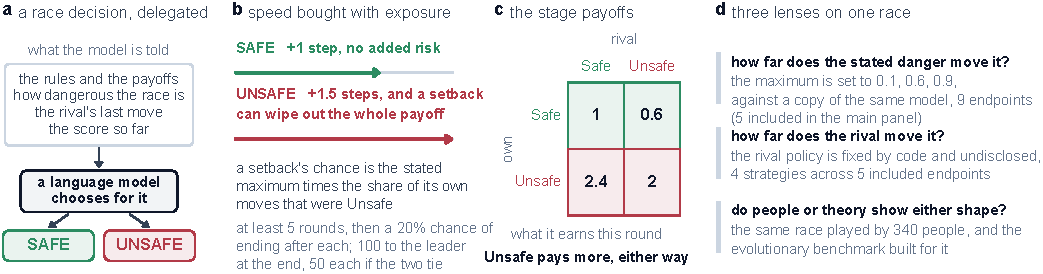
\includegraphics[width=\textwidth]{../../figures/paper/delegation_overview.pdf}
  \caption{The game and the questions it lets us ask. (a) The model receives
  the rules, stated danger, rival's last move and current score, then returns
  either \Safe{} or \Unsafe{}. (b) \Safe{} advances one step without added
  risk; \Unsafe{} advances faster but raises the chance that the winner's
  payoff is wiped out. (c) The two-player stage-payoff matrix makes \Unsafe{}
  attractive against either rival move, so the delayed terminal risk supplies
  the safety tension. (d) The main results examine stated-risk response,
  scripted-rival response, and comparison with human trajectories and the
  evolutionary benchmark.}
  \label{fig:mechanism}
  \Description{Four-panel overview of the AI development race. Panel a shows
  the information given to a language model and its Safe or Unsafe decision.
  Panel b shows the speed gained by Unsafe and the delayed private setback
  risk, together with the hidden horizon and terminal prize. Panel c shows the
  two-by-two stage-payoff matrix with own action as rows and rival action as
  columns. Panel d lists the three empirical lenses: stated danger, scripted
  rival, and the human and evolutionary references.}
\end{figure*}


\subsection{Two-player game}
\label{sec:prelim-2p}

Two companies $i \in \{1,2\}$ play a repeated race. In every round $t$, both simultaneously choose an action $a_i^t \in \{S, U\}$ (Safe, Unsafe) and commit to it before either learns the other's choice, and only then does the round resolve (Figure~\ref{fig:mechanism}a). Resolution has two parts. First, progress accumulates as $P_i^t = P_i^{t-1}+\sigma(a_i^t)$ with $\sigma(S)=1.0$ and $\sigma(U)=1.5$, so Unsafe always closes the race faster. Second, the round pays a stage payoff $\pi_i^t=\pi(a_i^t,a_{-i}^t)$, read off the fixed matrix (own action by row, opponent action by column, Figure~\ref{fig:mechanism}c):
\begin{equation}
    \pi = \begin{pmatrix} 1.0 & 0.6 \\ 2.4 & 2.0 \end{pmatrix}.
    \label{eq:2p-matrix}
\end{equation}
Unsafe strictly dominates Safe at the stage level (row 2 exceeds row 1 in both columns): the only cost of Unsafe development enters later, through accumulated private risk.

The race lasts a minimum of $5$ rounds; after every completed round from round $5$ onward it terminates with probability $0.2$, giving an expected horizon $\mathbb{E}[T]=9$. Neither company is ever told the horizon, so neither can condition on the current round being the last (Figure~\ref{fig:mechanism}a). Termination resolves in two further steps. First, the company with the higher cumulative progress $P_i^T$ wins a prize $B=100$, split $50/50$ on an exact tie. Second, and only for that winner or tied winners, an accumulated private setback risk is drawn:
\begin{equation}
    q_i(T) = p_r^{\max} \cdot \frac{n_i^U(T)}{T},\qquad p_r^{\max}\in\{0.1,0.6,0.9\},
    \label{eq:risk}
\end{equation}
where $n_i^U(T)$ counts company $i$'s Unsafe choices over the whole race and $p_r^{\max}$ is a treatment-level constant, assigned once per race, that we vary across three risk levels. If the draw against $q_i(T)$ fails, that company's entire race payoff, accumulated stage payoffs plus the prize, is zeroed. A company that ends behind is never subject to the draw: it keeps its stage payoffs regardless of how much Unsafe it played, but receives no share of the prize (Figure~\ref{fig:mechanism}a). This asymmetry, in which risk is built by both companies but realised only against whoever is ahead, is what makes Unsafe development a genuine gamble rather than a free speed advantage.

\subsection{Game-theoretic benchmark}
\label{sec:theory-benchmark}

\begin{table}[t]
\caption{The four benchmark strategies. Each is fixed by its opening move and
by what it does afterwards, so AS and AU never react to the other player while
CS and CAS react to nothing else. These four are also the fixed rivals of
\S\ref{sec:results-scripted}.}
\label{tab:benchmark-strategies}
\centering
\footnotesize
\setlength{\tabcolsep}{3pt}
\begin{tabular}{@{}llp{0.30\linewidth}@{}}
\toprule
Strategy & Opening & Every later round \\
\midrule
Always Safe (AS) & \Safe{} & \Safe{} \\
Cond.\ Safe (CS) & \Safe{} & copy the rival's last move \\
Cond.\ Antisocial Safe (CAS) & \Unsafe{} & copy the rival's last move \\
Always Unsafe (AU) & \Unsafe{} & \Unsafe{} \\
\bottomrule
\end{tabular}
\end{table}


The two incentives oppose each other. Stage-level dominance rewards Unsafe
immediately, while across the full race Unsafe choices raise the setback risk
for a winner or tied winner, so the best action can depend on the risk
condition, earlier actions, and the expected response of other players.

We use four simple strategies as a theory benchmark, defined in
Table~\ref{tab:benchmark-strategies}. Two of them ignore the other player and
two of them do nothing but answer it, which is what makes the set a benchmark:
it separates a fixed disposition from a reaction. In the reconstructed finite-population evolutionary model of
\citet{falling_behind_unsafe}, the most common strategy changes from AU at
$p_r^{\max}=0.10$, to CAS at $0.60$, and to CS at $0.90$: the theory predicts
not one fixed amount of Unsafe play but a risk-dependent shift between
unconditional speed, an aggressive opening and conditional restraint. We use
this as a qualitative benchmark, not as a fitted model of LLM output, because
prompted self-play trajectories are not samples from an evolutionary
population.
Selection strength $\beta$ controls how sharply payoff differences change
strategy frequencies: strong selection can create an abrupt switch, while weak
selection produces a more graded response. Mutation keeps alternative strategies
present. These are shape references, not mechanisms attributed to the endpoints.

\subsection{Best response to a fixed rival}
\label{sec:best-response}

Against a rival whose policy is fixed, the race is a single-agent decision
problem, and we solve it exactly by dynamic programming over the round, the
progress gap and the agent's own Unsafe count. The solver maximises expected
total payoff, so it is risk neutral, and it knows the rival's policy, which the
endpoints are never told. A 6{,}000-race simulation in the game engine
reproduces its payoffs and Unsafe rates (largest $|z|$ of 1.5).
Table~\ref{tab:best-response} gives the resulting Unsafe rates. Against
Always Safe the first move is an exact tie, so Unsafe play there is indifferent
rather than chosen, and the rival contrast below is the same under every tie
rule we tried (supplement S5.2).

\begin{table}[t]
\caption{Unsafe rate of the informed best response to each fixed rival, in percent,
by stated risk. The Always-Safe row is a tie at the first move, shown under one
tie rule.}
\label{tab:best-response}
\centering
\footnotesize
\setlength{\tabcolsep}{2pt}
\begin{tabular}{@{}lrrr@{}}
\toprule
Rival & Risk 0.1 & Risk 0.6 & Risk 0.9 \\
\midrule
AS  & 55.6 & 11.1 & 11.1 \\
CS & 55.6 & 55.6 & 33.7 \\
CAS & 100.0 & 55.3 & 51.4 \\
AU & 100.0 & 99.4 & 88.9 \\
\bottomrule
\end{tabular}
\end{table}

The best response therefore predicts a positive rival contrast. The best-response
Always-Unsafe minus Always-Safe contrast is $+44.4$, $+88.3$ and $+77.8$ points
at risks $0.1$, $0.6$ and $0.9$, and its rival-by-risk interaction is $+33.3$
points. A positive contrast and a positive interaction are what an informed best
responder does, so we do not present them as surprising. Two limits apply. The benchmark is
risk neutral and knows the rival's policy, which the endpoints must infer, so it marks a
reference point and not what an endpoint ought to play. A noisy best responder,
one that picks actions with probability rising in their value, can produce the
opposite sign. We therefore fit one for each endpoint: a logit quantal response
to the same rival, whose single noise parameter $\lambda$ is estimated by maximum
likelihood from the endpoint's own decisions at their recorded states, and we
predict its interaction by simulating that policy on the same seeds (supplement
S5.4). At the fitted noise, this benchmark predicts a negative interaction for
every endpoint. The two benchmarks therefore bracket the possible signs, and an
endpoint can be read against both.

\section{Experimental design and evidence policy}
\label{sec:design}
\subsection{Agent protocol and units of analysis}

At each decision an agent receives a versioned prompt carrying the round, the assigned maximum private risk, the disclosed state, and the preceding revealed action profile when $t>1$. Same-round decisions are sealed: every response comes from the same pre-action snapshot, before the engine resolves actions, progress, payoffs and risk, so the environment rather than generated text determines all transitions. Raw response, parsed action, retry and parser status, pre-turn state, terminal record, configuration and seed allocation are retained for every decision.

Sampling parameters here are provider-visible contracts, not intended
settings. The run manifests record a requested temperature of 0.7 that the
hosted SDK forwarded on no baseline endpoint, and no provider confirmed an
effective value. Seed handling was endpoint-specific: the SDK stripped the
requested seed on the Google endpoints and forwarded it, application
unconfirmed, on the OpenAI and Anthropic ones.

Both seats of a race are the same endpoint, so every gameplay rate below is
mirror-match play, until \S\ref{sec:results-scripted} fixes the rival instead.
For endpoint $m$, stated risk $p$ and rival policy $\pi$, define
\begin{equation}
    R_m(p,\pi)=\Pr_m(\Unsafe{}\mid p,\pi).
    \label{eq:opponent-conditioned-risk}
\end{equation}
Self-play observes only $R_m(p,m)$. The scripted-rival campaign instead compares
$R_m(p,\pi)$ across policies $\pi$ fixed by code, and its rival-by-risk estimand
is the change from low to high risk in the paired Always-Unsafe minus Always-Safe
contrast, which we compare with the best response of
\S\ref{sec:best-response}.

The main outcome is whether an agent chooses \Unsafe{}. A race is the independent
unit because later decisions depend on earlier states. We pool decisions only
when reporting a cell's rate. For comparisons, we first calculate the difference
within each matched repetition and then average those differences, so every
repetition receives equal weight. Intervals for rival contrasts and interactions
are BCa bootstrap intervals over the ten matched blocks, so they rest on ten
clusters. We also report sign-flip tests over the blocks, Holm-adjusted across
the five interactions, and a logit with cluster-corrected errors for the log-odds scale. Other
intervals are percentile bootstrap intervals over matched blocks. A \emph{parse failure} is a response outside
the required action format; because the fallback changes later states, it marks
the whole race as contaminated.
\subsection{Evidence strata and admission}

We separate two evidence strata and never pool them. A \emph{diagnostic pilot}
is an exploratory test for possible effects or failures; it does not estimate a
stable effect. A \emph{confirmatory} run here means that its protocol, endpoint,
prompt, configuration, race count and exclusion rules were fixed in the run
manifest when it started. It was not preregistered. The screen verdicts for
three of nine routes, which came after their gameplay, and the final three
GPT-5.5 scripted cells, collected after a declared change in the collection schedule, are not
called confirmatory.

One presentation check is described in the supplementary material: on two
endpoints, a fully crossed rerun retells the same game under a race story or as
an abstract contest, and substitutes the opaque response codes $P$ and $Q$ for
\Safe{} and \Unsafe{} under both code mappings. A task-validity screen gates
which endpoints enter the behavioural comparison. It is an inclusion rule, not
a behavioural outcome, and all gameplay results below are analysed without
ranking endpoints by its scores.

\subsection{Quality-control screen on the endpoints}
\label{sec:design-screen}

An action that parses is not evidence that the agent followed the race. Before
behavioural analysis, each endpoint therefore answered the same frozen bank of 20
probes over six task-validity domains, three times. An endpoint entered the study
only if it cleared the fixed thresholds of 80\% overall accuracy, 75\% state
reconstruction and 75\% terminal scoring. Five of nine endpoints passed; the
other four still played the same confirmatory baseline and remain available
throughout the trajectory-diversity analyses for transparency and sensitivity
checks.

The bank and operational thresholds were fixed before the campaign, and the
screen reads probes rather than races, so gameplay cannot change its verdict. It
was not preregistered: three of nine routes received their first verdict after
their gameplay had been collected. The admitted and refused groups split exactly
by the absence or presence of \texttt{mini}, \texttt{nano} or \texttt{lite} in
the route name, so the screen is in effect a size proxy. Two admitted endpoints
clear one domain at the minimum attainable passing score, and lowering state
reconstruction by one answer, from 75\% to 73.3\%, admits Gemini 3.1 Flash Lite.
The cutoffs are not externally validated. We therefore use the screen only as
an operational inclusion rule, never as a measure of comprehension, capability
or behaviour. The scripted-rival results cover the five admitted endpoints
only, so they do not show whether this exclusion changes them. The supplement
retains every route and score, and the stability of the admitted set.

\section{Results}
\label{sec:results}

Self-play supplies the baseline; the main result tests whether its risk
response survives a fixed opponent. Full tables and further checks are in
the supplement.

\subsection{Self-play suggests a shared directional risk response}
\label{sec:results-risk}

There is a shared directional response across the eligible endpoints. \Unsafe{}
play is non-increasing with the stated maximum private risk on every eligible
endpoint, while the shape varies: four of the five give ground gradually and the
fifth switches (Figure~\ref{fig:risk-response}). Each endpoint supplied 30 races
and 558 dependent within-race decisions under one frozen protocol, with zero
parse failures and ten races per risk cell. Risk contrasts use matched repetition
blocks, and race-weighted reanalysis preserves the low-to-high-risk contrast on
every eligible endpoint (supplementary material).

\begin{figure}[t]
    \centering
    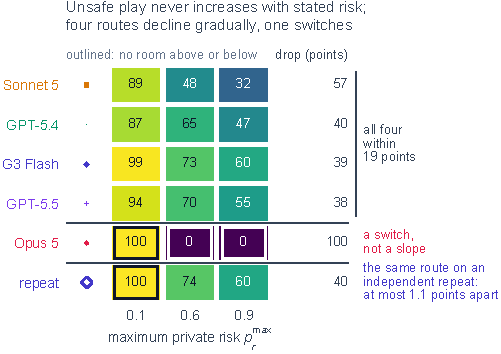
\includegraphics[width=\columnwidth]{../../figures/paper/risk_response.pdf}
    \caption{\Unsafe{} play is non-increasing with stated risk. The four graded
    endpoints fall within a 19-point band; Claude Opus 5 switches from the ceiling
    to the floor. The outlined cells are at a
    boundary and therefore leave no room for a larger or smaller observed
    rate. The repeat row is the same Gemini 3 Flash endpoint collected under an
    independent administration.}
    \label{fig:risk-response}
    \Description{Heatmap of Unsafe play for five eligible endpoints across three
    maximum private-risk conditions, with a right-hand column showing the drop
    from the lowest to the highest condition. Four graded endpoints lie in a
    narrow band and Claude Opus 5 forms a separate switch row; an additional
    repeat row is shown below.}
\end{figure}

The four graded endpoints, spanning three providers, have risk-response drops
from 38.2 to 57.0 percentage points. We report that band rather than a
five-endpoint average, which the switching endpoint would distort.

That fifth endpoint follows a threshold-like policy. Claude Opus 5 plays \Unsafe{}
on all 186 decisions at risk $0.1$ and \Safe{} on all 372 decisions above it,
with no race inside a cell departing from that. Its 100-point figure reaches
the largest value on the scale, and because no risk level was run between
$0.1$ and $0.6$, the location of its transition is not measured.

Even at the highest risk, the graded endpoints still play \Unsafe{} on a
third to three fifths of their decisions against a copy of themselves.

Repeating the whole protocol on Gemini 3 Flash with the same seeds and horizons
moved no risk cell by more than 1.1 points, against a 93.0-point spread in risk
response across the nine endpoints. This is a floor that excludes game variance;
collections on new seeds two months apart differ by up to 14 points.

Representation-equivalent prompt changes also move rates. The directional risk
response survives a fully crossed narrative-by-symbol rerun on two endpoints,
but equivalent renderings shift average \Unsafe{} play by 3.4 to 10.8
percentage points, and single cells move far more: on Gemini 3 Flash at risk
$0.9$ the four renderings give 43.5\% to 89.2\%. Neither the action-code
mapping nor the narrative skin is behaviourally inert (supplement S4). The mapping effect replicates across the two providers,
while the story effect differs, which warns against treating two endpoints as a
population of models. Because the rival campaign below uses one rendering, its
magnitudes and endpoint-specific shapes are conditional on it.

\begin{figure*}[t]
  \centering
  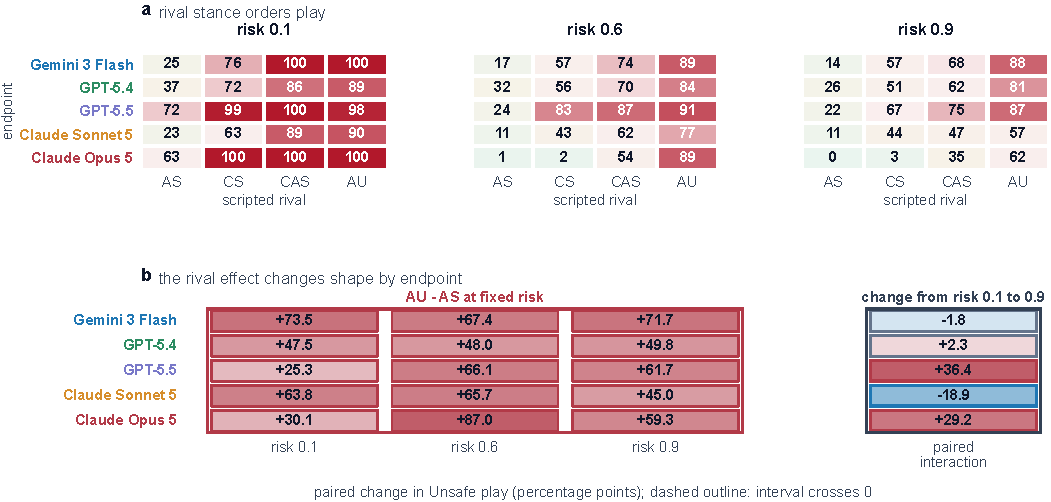
\includegraphics[width=\textwidth]{../../figures/paper/scripted_opponent_main.pdf}
  \caption{Changing the scripted rival changes \Unsafe{} play on every eligible
  endpoint. (a) Tiles show rates against four rivals at each risk level. (b)
  Larger tiles show the paired Always-Unsafe minus Always-Safe effect; every
  corresponding 95\% interval excludes zero. The right column gives the paired
  change in that effect from risk 0.1 to 0.9; solid outlines exclude zero and
  dashed outlines do not. Comparisons are within endpoints because endpoint
  settings differ. For reference, the informed best response gives a paired
  Always-Unsafe minus Always-Safe effect of $+44.4$, $+88.3$ and $+77.8$ points
  at risks 0.1, 0.6 and 0.9.}
  \Description{Two-panel figure. Panel a contains three response matrices,
  one per risk level, with five endpoint rows and four ordered scripted-opponent
  columns; every tile prints the measured Unsafe rate. Panel b contains five
  endpoint rows. Three red tiles per row show the paired Always Unsafe minus
  Always Safe effect at each risk, and a final signed tile shows how that effect
  changes from risk 0.1 to 0.9. Solid outlines mark intervals that exclude zero;
  dashed outlines mark intervals that cross zero.}
  \label{fig:scripted-opponent-main}
\end{figure*}

\subsection{Fixed rivals against the best response}
\label{sec:results-scripted}

Every rate so far is mirror-match play, in which the rival is the endpoint.
We now fix the rival in code. Five eligible endpoints each
played the four benchmark strategies of \S\ref{sec:theory-benchmark} at all
three risk levels: 60 cells, ten races each, 600 races and 5{,}580 endpoint
decisions with no parse failure anywhere. The rival's identity is never disclosed, and all 5{,}580 rival moves were
recomputed from the recorded history without a deviation. The endpoint's seat is counterbalanced five and five inside each cell, and
each contrast is taken inside a repetition, so the hidden horizon is differenced
out. Because the rival policy is assigned exogenously within matched blocks, the
direction of a rival-policy difference is identified.

All five tested endpoints respond to the scripted opponent policy. \Unsafe{} play
rises from the rival that always plays \Safe{}, through the two conditional
rivals, to the rival that never plays \Safe{}, in fourteen of fifteen
endpoint-by-risk cells, with strict ordering in twelve. The one reversal is
GPT-5.5 at risk $0.1$, where the CAS rival draws $100.0\%$ and
Always Unsafe is $97.8\%$, so this is a boundary case rather than a clean
counterexample (Figure~\ref{fig:scripted-opponent-main}a). The paired
difference between the two unconditional rivals is
positive in every cell, as the best response predicts. All fifteen paired-block
95\% intervals have positive lower bounds, with the smallest at $+16.5$ points
(Figure~\ref{fig:scripted-opponent-main}b). Adjusted for the fifteen tests, every
sign-flip $p$ value is 0.029, the smallest that ten blocks allow. The response to
the stated risk survives the change of design as well: against a fixed safe
rival, no endpoint's \Unsafe{} rate rises as the stated risk rises.

The size of the contrast is where the endpoints differ from the best response.
In 12 of the 15 cells the observed contrast is 10 or more points away from the
best-response value, and for no endpoint do more than 2 of its 12 rival-by-risk
cell rates fall inside the best-response range (none for Claude Sonnet 5 and
GPT-5.4).

\begin{table}[t]
\caption{Does stated risk change the rival effect? Entries are the paired
interaction $[(\mathrm{AU}-\mathrm{AS})_{0.9}-(\mathrm{AU}-\mathrm{AS})_{0.1}]$
in percentage points. Block A is the first collection (ten matched blocks, BCa
intervals); A+B adds a second collection on new seeds two months later (twenty
blocks, sign-flip intervals, Holm-adjusted $p$ of $0.049$ for Gemini 3 Flash,
$0.66$ for GPT-5.4 and below $0.001$ for both Claude endpoints). The last column is the interaction predicted by each endpoint's fitted noisy
best response (A+B; block A for GPT-5.5, whose second block is incomplete). Positive values mean that changing the rival
matters more at high risk; the last row is the informed best response. Contracts are not identical: GPT-5.5 and Claude Opus 5 ran with reasoning set
to low and a 1{,}024-token cap (one block-A Opus cell on an earlier contract);
Gemini 3 Flash, GPT-5.4 and Claude Sonnet 5 ran with reasoning off, at 256
tokens in block A and 1{,}024 in block B.}
\label{tab:rival-risk-interaction}
\centering
\scriptsize
\setlength{\tabcolsep}{3pt}
\setlength{\tabcolsep}{2pt}
\begin{tabular}{@{}lrrr@{}}
\toprule
Endpoint & Block A (pp) & A+B (pp) & Noisy BR \\
\midrule
Gemini 3 Flash  & $-1.8$ [$-8.9$, $2.9$] & $-4.7$ [$-8.7$, $-0.7$] & $-14.3$ \\
GPT-5.4         & $+2.3$ [$-4.6$, $9.7$] & $+1.1$ [$-3.9$, $6.0$] & $-1.4$ \\
GPT-5.5         & $+36.4$ [$29.3$, $44.3$] & incomplete & $-16.9$ \\
Claude Sonnet 5 & $-18.9$ [$-24.4$, $-10.8$] & $-25.9$ [$-30.9$, $-20.7$] & $-24.1$ \\
Claude Opus 5   & $+29.2$ [$19.2$, $35.4$] & $+22.3$ [$14.6$, $29.9$] & $-18.8$ \\
\midrule
Informed best response & $+33.3$ & $+33.3$ & \\
\bottomrule
\end{tabular}
\end{table}

Table~\ref{tab:rival-risk-interaction} sets each endpoint's interaction beside
both benchmarks. We call an endpoint consistent with a benchmark when its
observed interaction lies inside that benchmark's 95\% band. Claude Sonnet 5's
interaction is negative in both collection blocks and pooled ($-25.9$ points,
Holm $p<0.001$), and its fitted noisy best response predicts almost exactly that
($-24.1$, band $-36.8$ to $-11.3$). Gemini 3 Flash and GPT-5.4 are near zero:
inside their noisy bands when the blocks are pooled, but also compatible with no
interaction, and far from the informed best response. Claude Opus 5 and GPT-5.5
are positive ($+22.3$ and $+36.4$) where their fitted noise predicts $-18.8$ and
$-16.9$, so they respond to the rival as sharply as the informed benchmark, a
sign this noise model cannot produce. Opus's sign holds on the rate scale but
not on the log-odds scale, where its ceiling and floor cells make the estimate
unstable ($-1.13$, 95\% interval $-2.29$ to $0.04$). The noisy benchmark is
fitted in-sample, one parameter per endpoint, on the same decisions it is then
compared with.

The two positive endpoints are also the two that run with reasoning enabled and
a 1{,}024-token cap, so the contract is a candidate cause. It is not sufficient:
Claude Sonnet 5 run under that same contract becomes much less noisy ($\lambda$
rises from $0.10$ to $0.45$), its noisy benchmark then predicts no interaction
($+0.1$, band $-14.1$ to $+14.0$), and it plays $-35.2$ points, departing from
both benchmarks in the negative direction. A model that conditions on the race
position and a fitted belief about the rival, but not on the rival's observed
moves, fits four of five endpoints better than the noisy best response,
although it has more freedom; most endpoints thus appear to react to the race
state the rival creates rather than to a model of the rival (supplement S5.4).
The interaction was not re-measured under the other prompt renderings, which
move single cells by up to 46 points, so its size is specific to this
rendering. The blocks differ by up to 14 points for the same endpoint, which
fits provider-side change between collections (supplement S5.3).

The two conditional rivals make the dependence visible at the first move. They
follow the same policy from round two onward and differ only in whether the rival
opens \Safe{} or \Unsafe{}. That opening-move contrast has a positive lower 95\%
bound in twelve of fifteen endpoint-by-risk cells, showing that one exogenous
rival action can redirect the later path.

A mirror-match rate is therefore the outcome of one policy meeting itself,
not a stand-alone measurement of how an endpoint treats risk. For Gemini 3
Flash, the self-play profile is $98.9\%$, $73.1\%$ and $60.2\%$, whereas the
same endpoint against Always Safe gives $24.7\%$, $17.2\%$ and $14.0\%$.
Self-play exceeds the fixed-safe rate in thirteen of fifteen cells, with the two
exceptions for Claude Opus 5 at the floor ($0.0\%$ against $1.1\%$ at risk
$0.6$, and a $0.0\%$ tie at risk $0.9$). This is close to mechanical: the mirror
rival is an adaptive policy, not a fixed-safe one, so the comparison motivates
the fixed-rival design rather than supporting it.




\subsection{Shape against an evolutionary benchmark}
\label{sec:results-theory}

The graded endpoint profiles are closer to a weak-selection setting of the
reconstructed model of \citet{falling_behind_unsafe} than to its strong-selection
reference. Gemini 3 Flash gives 98.9\%, 73.1\% and 60.2\% over 30 races, and
Claude Sonnet 5 gives 89.2\%, 48.4\% and 32.3\%. At the reference setting
($\beta=2$, $\mu=\beta/Z$) the model loses 98 points inside a risk step of
$0.005$, a step none of the graded endpoints shows. We swept 90 settings of
selection strength and mutation rule and kept the closest cell, chosen as the
best of 90 over three risk points. It is $\beta=0.01$, $\mu=0.05$, which are
also the source study's human-fitted values. There the model predicts 87.3\%,
63.9\% and 38.0\%, within 9.6 points of Claude Sonnet 5 and 15.4 of Gemini 3
Flash in root-mean-square error. All five endpoints have lower error at this
cell than at the reference setting, with Claude Opus 5 the near-step exception.
A drift-dominated regime is graded by construction, so this shows that the
endpoint shapes are not strong-selection shapes, not that the model explains
them. The sweep, its figure and the endpoint-level errors are in supplement S3.

\subsection{Repeated endpoint samples occupy fewer paths than human samples}
\label{sec:results-diversity}

One endpoint sampled repeatedly under one decoding setting is compared here with
many different people, so fewer distinct paths is expected of any single policy.
We treat the result as a descriptive contrast, not as a second failure of
aggregate evaluation. We compare exact first-five-round joint-action
trajectories, represented as ten-bit strings, over 60 trajectories per endpoint
from the baseline campaign (20 per risk level, two seat views of ten races). The only human
reference is the de-identified dataset of \citet{falling_behind_unsafe}, so the
comparison is bounded to that population and game. Its primary null uses 168
complete dyads.

Two endpoints that failed the screen, GPT-5.4 mini and nano, fall inside the
human range under the participant-level sensitivity, so the contrast does not
hold for every endpoint. Each endpoint sample is compared with $20{,}000$
equally sized resamples of ten complete human dyads at each risk. Whole dyads
preserve the interaction, and equal sample sizes stop the larger human dataset
from gaining an automatic advantage. Eighteen of 27 endpoint cells, including 13
of the 15 eligible cells, fall below every dyad draw, and GPT-5.4 and GPT-5.5 do
not at risk $0.9$. A participant-level sensitivity places all 15 eligible cells
below every draw, and under the effective trajectory count \citep{hillDiversity1973}
every eligible endpoint sits below the human interval at every risk level.
Measured as a gap, every eligible cell lies below the central 95\% of the
matched human draws, with 5.2 to 18.6 fewer distinct trajectories out of 20
than the mean draw (median 12.2).

The concentration is strongest for Claude Opus 5, which produces a single
trajectory, repeated by all 20 of its trajectories at each risk level, while
Claude Sonnet 5 uses two at risk $0.1$. Concentration is also distinct from
level: Gemini 3 Flash and GPT-5.5 finish within five points of each other at the
highest risk and use 12 and 13 distinct trajectories, yet the Gemini trajectories
sit half again as far apart, 0.41 against 0.27 in mean pairwise distance. The
three-panel figure, the rank-frequency view and the modal sequences are in
supplement S6.

\section{Discussion and conclusion}
\label{sec:discussion}

A self-play rate is not a stable trait of an endpoint. In self-play the
endpoint supplies both sides of the interaction, so its early actions create
the history its later actions respond to. Fixing the rival by code removes that
loop and lets us ask a sharper question: which benchmark does each endpoint
resemble when the rival is known to the analyst? A positive rival contrast is
what every benchmark predicts, so it is not the result. The rival-by-risk
interaction is, because an exact and a fitted noisy best response predict
opposite signs. Claude Sonnet 5 matches the noisy benchmark, Gemini 3 Flash and
GPT-5.4 are near zero, Claude Opus 5 and GPT-5.5 show the sign only a sharp
responder produces, and Claude Sonnet 5 with reasoning enabled matches neither. Each reading holds
within one endpoint and its own decoding contract.

The opponent can matter as much as the stated risk. Against the
Always-Safe rival, raising maximum private risk from $0.1$ to $0.9$ lowers
\Unsafe{} play by 10.4 to 69.9 percentage points across endpoints. At fixed
risk, replacing Always Safe with Always Unsafe raises it by 25.3 to 87.0 points.
The two spans overlap, so neither factor is always larger.

This changes what a strategic-agent evaluation should report. Self-play
estimates the outcome of two copies of one policy, a fixed rival estimates a
response conditional on that declared policy, and a mixed pool estimates
outcomes under its own population mix. We propose, without having validated it
beyond this game, that each endpoint be reported against an exact and a fitted noisy best
response for every declared rival, alongside a task-validity screen,
whole-trajectory measures and crossed presentation controls. Presentation
belongs in it because both the action-code mapping and the narrative skin moved
rates. The trajectory contrast is a descriptive reference, not a target: one
fixed policy is expected to occupy fewer paths than a population, and a match on
one measure does not imply a shared mechanism.

The scope is deliberately narrow. Nine commercial endpoints are not a model
population, decoding contracts differ across endpoints, and the scripted panel
uses four chosen policies. Both benchmarks are risk neutral and know the rival's policy, so they are
references for reading behaviour, not verdicts on rationality, and the noisy
benchmark has one free parameter fitted to the same data.
One Claude Opus 5 cell used an earlier decoding contract; re-collected under
the active contract it stays at the floor (4.3\% against 1.1\% \Unsafe{}). The interactions rest on
twenty matched blocks per endpoint at most, and the second block is a later
re-administration under a larger output cap, not an identical replication. Provider-side temperature and seed handling could not be confirmed, so
the closed endpoints cannot be regenerated exactly. The game omits collective
harm, regulation and communication, so the results say nothing about general
model safety or real organisations. An exploratory group-size study on one
endpoint is in the supplement. The most informative next tests are adaptive
rivals and cross-play, an open-weight replication with controlled decoding, a
denser risk grid around the observed switches, and the same matched design in a
second game.

Code, the de-identified run records and a checker that recomputes every
reported quantity are provided with the supplementary material and will be
released with the final version. The checker recomputes quantities from the
stored records; it does not re-query the closed endpoints.

% Acknowledgements name individuals, their institutions and a grant number, so
% they identify the authors. The class does not suppress this section in
% anonymous mode, it prints whatever is here. Restore the block below for the
% camera-ready, together with the non-anonymous \documentclass at the top.
%
% \section*{Acknowledgements}
% T.A.H. acknowledges travel and accommodation support from the Ho Chi Minh City University of Technology (HCMUT), VNUHCM (Adjunct Professorship scheme HCMUT\text{-}VNUHCM). L.H.T acknowledges the Ho Chi Minh City University of Technology (HCMUT), VNUHCM for supporting this study.
% TAH is supported by EPSRC (grant EP/Y00857X/1).
 
\section*{Use of AI Tools}
Claude Code and OpenAI Codex were used for code assistance, verification and
manuscript editing. Exact model versions and complete interaction histories were
not retained. The authors checked the resulting code and prose against the
archived evidence and take responsibility for the manuscript, analyses and
citations.

\clearpage
\bibliographystyle{named}
\bibliography{../references}

\end{document}
